\chapter{Análise dos Resultados}
\label{cap:04}

Foi desenvolvido as quatros versões do jogo \textit{Tetris} utilizando as tecnologias \textit{Godot}, \textit{Pygame}, \textit{Raylib} e \textit{LibGDX}, após a implementação, foi feita uma análise comparativa entre as tecnologias, levando em consideração aspectos como facilidade de uso, curva de aprendizado e desempenho.
Para a implementação do jogo \textit{Tetris} foi levantado os requisitos necessários para o desenvolvimento do jogo, como a movimentação das peças, a rotação, a queda automática, o sistema de colisão e a remoção de linhas completas.

\section{Estudos das Tecnologias e Implementação}

Antes do desenvolvimento de cada versão do jogo, foi realizado um estudo introdutório da linguagem de programação utilizada pela tecnologia correspondente, buscando compreender conceitos fundamentais de sintaxe, orientação a objetos, manipulação gráfica e estrutura de execução.

Após o estudo introdutório da linguagem, foi feito um estudo da documentação oficial de cada engine ou biblioteca/\textit{Framework}, com foco nos recursos necessários para o desenvolvimento do jogo \textit{Tetris}, como renderização gráfica, captura de entrada do usuário, temporização e o gerenciamento de desenho de elementos.

O desenvolvimento foi realizado de forma incremental e comparativa. A cada nova implementação, aplicou-se os mesmos requisitos do jogo em diferentes ambientes de desenvolvimento. Essa abordagem possibilitou observar diferenças relacionadas à organização do código, gerenciamento do loop principal do jogo, modularização e disponibilidade de recursos oferecidos por cada tecnologia. Durante esse processo, também foram estudados e incorporados algoritmos e mecânicas adicionais presentes no \textit{Tetris}, como o sistema de geração de peças \textit{7-Bag} (para evitar peças iguais) e o \textit{Super Rotation System} (SRS) (sistema de rotação para cada peça), possibilitando a evolução gradual das implementações ao longo do projeto.

Nas subseções abaixo serão mostradas como algumas funções essênciais foram implementadas de acordo com cada linguagem e tecnologia.


\subsection{Godot}

Durante o desenvolvimento do jogo na \textit{Godot}, observou-se uma grande facilidade na criação de cenas e gerenciamento de nós, permitindo uma implementação rápida da lógica do jogo. A estrutura de nós da \textit{Godot} facilitou a organização do código e a reutilização de componentes, o que contribuiu para uma implementação mais eficiente do jogo \textit{Tetris}. A documentação da \textit{Godot} foi útil para esclarecer dúvidas e fornecer exemplos práticos, acelerando o processo de desenvolvimento.

\subsubsection{Nós e Scripts}

Foi utilizado 2 nós principais para a implementação do jogo, o nó \textit{Node2D} para a cena principal do jogo e outro nó \textit{Node2D} para as peças do jogo, além de outros nós auxiliares para a temporização e gerenciamento gráfico, junto aos dois nós principais, foram criados scripts para implementar a lógica do jogo, como a movimentação das peças, a rotação, a queda automática, o sistema de colisão e a remoção de linhas completas.

Abaixo na figura~\ref{fig:godotnos}, estão os nós e os scripts criados para a implementação do jogo \textit{Tetris} na \textit{Godot}:
\FloatBarrier
\begin{figure}[!htbp]
	\centering
	\caption{Nós e Scripts do Jogo Tetris na Godot}
	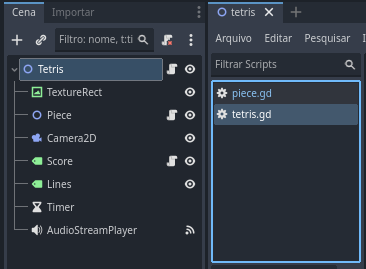
\includegraphics[scale=1.2]{imagens/Nos&Scripts.png}
	\\\textbf{Fonte:} Elaborado pelo autor
	\label{fig:godotnos}
\end{figure}
\FloatBarrier

Os dois scripts tem dentro deles outros nós, como o nó de temporização e os nós Label Score e Lines.

\subsubsection{Instanciação de Peças}

A função de surgir as peças do jogo, chamada de \textit{spawnPiece}, é implementada dentro do script do nó principal do jogo, o \textit{Node2D} da cena principal, e é responsável por criar uma nova peça e posicioná-la no topo do tabuleiro.

Abaixo está  implementado o código dessa função:
\lstinputlisting[language=]{fontes/Godot/spawnPieceGodot.gd} 

Como visto no código acima, a função \textit{spawnPiece} utiliza a função \textit{randi} para gerar um número aleatório entre 1 e 7, que corresponde a uma das sete peças do jogo \textit{Tetris}. Em seguida, ocorre uma condição que verifica se o espaço está disponível para a nova peça. Se sim, a função instancia a peça correspondente e a adiciona como filha do nó principal do jogo, senão, é chamada a função \textit{gameOver}. Por fim, a função posiciona a peça no topo do tabuleiro, utilizando as coordenadas do meio do tabuleiro para centralizá-la horizontalmente e colocá-la no topo do tabuleiro.
É importante observar que há possibilidade de aparecer peças iguais em sequência.
Sempre quando uma peça é travada no tabuleiro, a função \textit{spawnPiece} é chamada para criar uma nova peça.

\subsubsection{Verificação e remoção de linhas}

Quando uma linha ou mais linhas na grade é completada, a função de remoção de linhas é chamada, \textit{cleanLines}, e é responsável por verificar quais linhas estão completas, removê-las do tabuleiro e atualizar a pontuação do jogador. 

Abaixo está implementado o código dessa função:
\lstinputlisting[language=]{fontes/Godot/cleanLinesGodot.gd}

A função \textit{cleanLines} percorre cada linha do tabuleiro, verificando se todas as células da linha estão ocupadas por peças. Se uma linha completa for encontrada, 
é chamada a função \textit{removeLine} para remover a linha do tabuleiro. A função \textit{removeLine} recebe o índice da linha a ser removida. Esse processo ocorre de baixo para cima. 

Abaixo está implementado o código da função \textit{removeLine}:

\lstinputlisting[language=]{fontes/Godot/removeLineGodot.gd}

A função \textit{removeLine} remove a linha do tabuleiro, iterando sobre as células da linha e recolocando as peças acima da linha removida para baixo.

A pontuação do jogador é atualizada com base no número de linhas removidas, seguindo a fórmula de pontuação tradicional do jogo \textit{Tetris}, onde a pontuação aumenta exponencialmente com o número de linhas removidas simultaneamente.

\subsubsection{Temporização e Queda Automática}

A temporização na \textit{Godot} é implementada utilizando o nó \textit{Timer}, que é adicionado na função interna \textit{ready}. O temporizador é configurado para disparar a cada 0.5 segundos, o que determina a velocidade de queda das peças. Abaixo está implementado o código para configurar o temporizador:

\lstinputlisting[language=]{fontes/Godot/timerGodot.gd}

A linha 7 conecta o temporizador e função responsável por fazer a peça cair \textit{fall}, simulando a queda automática.

Abaixo está implementado o código da função \textit{fall}:

\lstinputlisting[language=]{fontes/Godot/fallGodot.gd}

Nessa função, há uma variavel chamada \textit{checkFall} que é utilizada para verificar se a peça não pode cair, ou seja, se há colisão com o tabuleiro ou com outras peças. Se a peça não puder cair uma vez em 0.5 segundos, é adicionado 1 na variável \textit{checkFall}. Se a variavel estiver com o valor 2, é chamada a função \textit{lockPiece} para travar a peça no tabuleiro, a função para verificar se há linhas completas e a função \textit{spawnPiece} para criar uma nova peça e o valor da variável \textit{checkFall} é resetado para 0.

\subsubsection{Movimentação}

A movimentação das peças é implementada utilizando a função de captura de entrada do usuário, que é chamada dentro da função \textit{process}, responsável por atualizar o estado do jogo a cada frame. Abaixo está implementado o código para capturar a entrada do usuário:

\lstinputlisting[language=]{fontes/Godot/processGodot.gd}

Nessa função, são verificadas as teclas pressionadas pelo jogador para movimentar, rotacionar ou fixar a peça. A função de movimentação das peças, chamada de \textit{move}, é implementada dentro do script do nó das peças e é responsável por atualizar a posição da peça com base na entrada do usuário. Abaixo está implementado o código da função \textit{move}:

\lstinputlisting[language=]{fontes/Godot/moveGodot.gd}

Dentro da função \textit{move}, é verificado se a nova posição da peça é válida, ou seja, se não há colisão com o tabuleiro ou com outras peças. Se a posição for válida, a peça é movida para a nova posição, caso contrário, a peça permanece na posição atual. A função que faz essa verificação é a função \textit{isValidMove}, que é implementada dentro do script do nó das peças e é responsável por verificar se a peça colidiu com o tabuleiro ou com outras peças. Abaixo está implementado o código da função \textit{isValidMove}:

\lstinputlisting[language=]{fontes/Godot/isValidMoveGodot.gd}

Essa função checa os limites horizontais e verticais da grade, além de verificar se a posição da peça colidiu com outras peças. Se a posição for válida, a função retorna \textit{true}, caso contrário, retorna \textit{false}.

A função de rotação das peças, chamada de \textit{rotate}, também é implementada dentro do script do nó das peças, e é responsável por alterar a orientação da peça quando o jogador solicita uma rotação. Abaixo está implementado o código da função \textit{rotate}:

\lstinputlisting[language=]{fontes/Godot/rotateGodot.gd}

\subsection{LibGDX}

A implementação do jogo \textit{Tetris} na \textit{LibGDX} apresentou uma abordagem mais tradicional de desenvolvimento, utilizando a linguagem \textit{Java}, a IDE Visual Studio Code e os recursos da engine para implementar o Tetris.
Foi utilizado o paradigma de programação orientada a objetos para organizar o código, criando classes para representar as peças, o tabuleiro e a lógica do jogo. A \textit{LibGDX} forneceu uma boa estrutura para lidar com gráficos e entrada do usuário, mas exigiu um pouco mais de configuração inicial em comparação com a \textit{Godot}. A documentação da \textit{LibGDX} foi útil para entender os conceitos básicos e as funcionalidades da engine, mas em alguns momentos foi necessário recorrer a fóruns e tutoriais de terceiros para esclarecer dúvidas específicas relacionadas à implementação do jogo e à recursos da engine \textit{Tetris}.

\subsubsection{Classes}

Foi implementado 4 classes para que o jogo \textit{Tetris} fosse implementado, a classe \textit{Tetris} para a lógica principal do jogo e representar o tabuleiro do jogo, a classe \textit{Piece} para representar as peças do jogo, a classe \textit{InputProcessor} para lidar com a entrada do usuário e a classe \textit{Main} para gerenciar o fluxo principal do jogo, na figura~\ref{fig:libgdxclasses} é mostrado as classes criadas para a implementação do jogo \textit{Tetris} na \textit{LibGDX}:

\FloatBarrier
\begin{figure}[!htbp]
	\centering
	\caption{Classes do Jogo Tetris na LibGDX}
	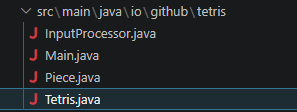
\includegraphics[scale=1.2]{imagens/ClassesLibGDX.png}
	\\\textbf{Fonte:} Elaborado pelo autor
	\label{fig:libgdxclasses}
\end{figure}
\FloatBarrier

Todas as classes tem dentro delas uma instância do objeto da classe \textit{Tetris}, que é a classe principal do jogo, para que possam acessar os métodos e atributos da classe.
Dentro da classe \textit{Tetris} tem uma instância da classe \textit{Piece} para utilizar os métodos e atributos da classe \textit{Piece} e para o travamento das peças no tabuleiro. %Pode escrever travamento?????? não sei como escrever de outra forma
A classe \textit{Main} gerencia o fluxo principal do jogo, como a renderização gráfica, a captura de entrada do usuário e a temporização.

\subsubsection{Gerar peças}

A função de gerar as peças do jogo, em comparação com a implementação na \textit{Godot}, é implementada de uma forma diferente e mais eficiente, para evitar peças iguais. Dentro da classe \textit{Tetris} tem a função \textit{spawnPiece}, que é responsável por criar uma nova peça e posicioná-la no topo do tabuleiro. Abaixo está implementado o código dessa função:

\lstinputlisting[language=Java]{fontes/LibGDX/spawnPieceLibGDX.java}

A função \textit{spawnPiece} tem uma lógica diferente da função de gerar peças da implementação na \textit{Godot}, para evitar peças iguais, o numero para pegar a peça é gerado utilizando um sistema de \textit{7-Bag}. O sistema de \textit{7-Bag} é como se fosse um saco com as sete peças do jogo \textit{Tetris}, onde cada peça é retirada do saco de forma aleatória, garantindo que todas as peças sejam geradas antes de repetir qualquer peça. Abaixo está implementado o código do sistema de \textit{7-Bag} em 2 funções, a função \textit{refillPieceQueue} e a função \textit{getNextPieceNum}:

\lstinputlisting[language=Java]{fontes/LibGDX/7Bag.java}

Há um array de inteiros chamado \textit{bagPieces} que a função \textit{getNextPieceNum} remove sempre o primeiro elemento da lista e retorna esse elemento como o número da peça a ser gerada. Quando a lista de peças do saco (\textit{bagPieces}) estiver vazia, a função \textit{refillPieceQueue} é chamada para preencher o saco com as sete peças do jogo, embaralhando com o \textit{Collections.shuffle} a ordem das peças para garantir aleatoriedade.

\subsubsection{Verificação e remoção de linhas}

Segue a mesma lógica da implementação na \textit{Godot}, a função de remoção de linhas é chamada sempre quando uma peça é colocada, \textit{cleanLines}, e é responsável por verificar quais linhas estão completas, removê-las do tabuleiro e atualizar a pontuação do jogador. Abaixo está implementado o código das 2 funções, a função \textit{cleanLines} e a função \textit{removeLine}:

\lstinputlisting[language=Java]{fontes/LibGDX/cleanLine.java}

A função \textit{clean} percorre cada linha do tabuleiro, verificando se todas as células da linha estão ocupadas por peças. Se uma linha completa for encontrada, é chamada a função \textit{removeLine} para remover a linha do tabuleiro. A função \textit{removeLine} recebe o índice da linha a ser removida. Esse processo ocorre de baixo para cima. A função \textit{removeLine} remove a linha do tabuleiro, iterando sobre as células da linha e recolocando as peças acima da linha removida para baixo.

\subsubsection{Temporização}

Abaixo está parte do código implementado para configurar a temporização do jogo, utilizando a função \textit{render} da \textit{LibGDX} para atualizar o estado do jogo a cada frame:

\lstinputlisting[language=Java]{fontes/LibGDX/render.java}

Nessa função, a variável \textit{fallTimer} é incrementada com o tempo decorrido desde o último frame, utilizando o método \textit{Gdx.graphics.getDeltaTime} para obter o tempo em segundos. Quando o \textit{fallTimer} atinge ou ultrapassa o valor definido em \textit{fallInterval} (0.5 segundos), o temporizador é resetado para zero e a função responsável por fazer a peça cair, chamada de \textit{canfall}, é chamada para simular a queda automática das peças. Junto também tem a variável \textit{lockTimer} que é utilizada para verificar se a peça não pode cair, ou seja, se há colisão com o tabuleiro ou com outras peças. Se a peça não puder cair uma vez em 0.5 segundos, é adicionado 1 na variável \textit{lockTimer}. Se a variavel estiver com o valor maior que o limite \textit{lockDelay}, é chamada a função \textit{lockPiece} para travar a peça no tabuleiro.


\subsubsection{Movimentação}

A movimentação das peças é implementada utilizando a classe \textit{InputProcessor} para lidar com a entrada do usuário, que é chamada dentro da função \textit{render}, responsável por atualizar o estado do jogo a cada frame. Abaixo está implementado o código para capturar a entrada do usuário:

\lstinputlisting[language=Java]{fontes/LibGDX/InputProcessor.java}

Nessa função, são verificadas as teclas pressionadas pelo jogador para movimentar, rotacionar ou fixar a peça. A função de movimentação das peças, chamada de \textit{move}, é implementada dentro da classe \textit{Piece} e é responsável por atualizar a posição da peça com base na entrada do usuário. Abaixo está implementado o código da função \textit{move}:

\lstinputlisting[language=Java]{fontes/LibGDX/move.java}

Dentro da função \textit{move}, é verificado se a nova posição da peça é válida, ou seja, se não há colisão com o tabuleiro ou com outras peças. Se a posição for válida, a peça é movida para a nova posição, caso contrário, a peça permanece na posição atual. A função que faz essa verificação é a função \textit{isValidMove}, que é implementada dentro da classe \textit{Piece} e é responsável por verificar se a peça colidiu com o tabuleiro ou com outras peças. Abaixo está implementado o código da função \textit{isValidMove}:

\lstinputlisting[language=Java]{fontes/LibGDX/isValidMove.java}

Essa função checa os limites horizontais e verticais da grade, além de verificar se a posição da peça colidiu com outras peças. Se a posição for válida, a função retorna \textit{true}, caso contrário, retorna \textit{false}.
A função de rotação das peças, chamada de \textit{rotate}, também é implementada dentro da classe \textit{Piece}, e é responsável por alterar a orientação da peça quando o jogador solicita uma rotação. Abaixo está implementado o código da função \textit{rotate}:

\lstinputlisting[language=Java]{fontes/LibGDX/rotate.java}

O método de rotação utilizado é uma versão simplificada do \textit{Super Rotation System} (SRS), que é um sistema de rotação para cada peça, onde cada peça tem um conjunto específico de regras para rotação, permitindo uma rotação mais fluida e intuitiva, especialmente em situações de colisão.
Caso a peça não possa ser rotacionada devido a uma colisão, o sistema de rotação tenta aplicar um deslocamento (chamado de "kick") para tentar encontrar uma posição válida para a peça rotacionada, é feito 4 tentativas. Se nenhuma posição válida for encontrada, a peça permanece na orientação atual.


\subsection{Raylib}

A implementação do jogo \textit{Tetris} na \textit{Raylib} apresentou uma abordagem mais direta e de baixo nível, foi utilizado tambem o Visual Studio Code como ambiente de desenvolvimento, usou-se a linguagem \textit{C++} e os recursos do \textit{Framework} para implementar o Tetris. A \textit{Raylib} forneceu uma boa estrutura para lidar com gráficos e entrada do usuário, mas exigiu um pouco mais de configuração inicial em comparação com a \textit{Godot} e a \textit{LibGDX}. A documentação da \textit{Raylib} foi útil para entender os conceitos básicos e as funcionalidades do \textit{Framework}, porém, em alguns momentos foi necessário recorrer a fóruns e tutoriais de terceiros para esclarecer dúvidas específicas relacionadas à linguagem \text{C++}, como por exemplo, o uso de ponteiros e referências.

Há tambem na documentação oficial exemplos prontos de implementação de jogos, incluindo uma versão funcional do jogo \textit{Tetris}. Entretanto, esse exemplo não foi utilizado diretamente no desenvolvimento do projeto, por que o objetivo do trabalho consistia em compreender e implementar manualmente as mecânicas do jogo, permitindo maior aprofundamento nos conceitos da linguagem \textit{C++} e da própria biblioteca.

\subsubsection{Classes}

Foi implementado 4 classes para essa versão, a classe \textit{Tetris} para a lógica principal do jogo e representar o tabuleiro do jogo, a classe \textit{Piece} para representar as peças do jogo, a classe \textit{Game} para gerenciar o fluxo principal do jogo, como a renderização gráfica, a captura de entrada do usuário e a temporização, e a classe principal presente em \textit{main.cpp}, utilizada para inicialização da implementação.
Além disso,a implementação utilizou arquivos de cabeçalho (\textit{headers}), como \textit{piece.h}, \textit{tetris.h} e \textit{game.h}, responsáveis pela declaração das classes, atributos e métodos utilizados no projeto. Já os arquivos com extensão \textit{.cpp} foram utilizados para a implementação da lógica dessas classes. Essa separação entre declaração e implementação contribuiu para uma melhor organização e modularização do código, característica comum em projetos desenvolvidos em \textit{C++}.

Como \textit{C++} requer um gerenciamento de memória manual, foi necessário lidar com a gestão de memória manualmente, utilizando ponteiros e referências para criar e destruir objetos dinamicamente.
Na figura~\ref{fig:raylibclasses} é mostrado as classes criadas para a implementação do jogo \textit{Tetris} na \textit{Raylib}:

\FloatBarrier
\begin{figure}[!htbp]
	\centering
	\caption{Classes e Headers do Jogo Tetris na Raylib}
	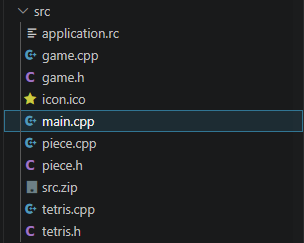
\includegraphics[scale=1.2]{imagens/ClassesRaylib.png}
	\\\textbf{Fonte:} Elaborado pelo autor
	\label{fig:raylibclasses}
\end{figure}
\FloatBarrier

\subsubsection{Gerar Peça}

O código para gerar as peças do jogo na \textit{Raylib} segue a mesma lógica da implementação da \textit{LibGDX}, utilizando o algoritmo \textit{7-bag}, que é implementado dentro da classe \textit{Tetris} e é responsável por criar uma nova peça e posicioná-la no topo do tabuleiro. Abaixo está implementado o código dessas funções:

\lstinputlisting[language=C++]{fontes/Raylib/spawnPiece.cpp}

Tem um array de inteiros chamado \textit{bagPieces}, é removido o último elemento da lista e retorna esse elemento como o número da peça a ser gerada. Quando a \textit{bagPieces} estiver vazia, a função \textit{refillBag} é chamada para preencher o saco com as sete peças do jogo, embaralhando com a função \textit{std::shuffle} a ordem das peças para garantir aleatoriedade.
Logo apos é verificado se o espaço está disponível para a nova peça. Se sim, a função instancia a peça correspondente, senão, o jogo é encerrado. É importante observar que foi utilizado ponteiros na hora de verificar o espaço, para que a verificação seja feita por referência e não por valor.

\subsubsection{Verificação e remoção de linhas}

A função de remoção de linhas também segue o mesmo princípio da implementação da \textit{LibGDX}. Ela é chamada sempre quando uma peça é colocada, \textit{cleanLines}, e é responsável por verificar quais linhas estão completas, removê-las do tabuleiro e atualizar a pontuação do jogador. Abaixo está implementado o código das 2 funções, a função \textit{cleanLines} e a função \textit{removeLine}:

\lstinputlisting[language=C++]{fontes/Raylib/cleanLines.cpp}

A função \textit{cleanLine} percorre cada linha do tabuleiro, verificando se todas as células da linha estão ocupadas por peças. Se uma linha completa for encontrada, é chamada a função \textit{removeLine} para remover a linha do tabuleiro. A função \textit{removeLine} recebe o índice da linha a ser removida. Esse processo ocorre de baixo para cima. A função \textit{removeLine} remove a linha do tabuleiro, iterando sobre as células da linha e recolocando as peças acima da linha removida para baixo.


\subsubsection{Temporização e Queda Automática}

Na implementação utilizando a \textit{Raylib}, a temporização foi realizada através da atualização contínua do estado do jogo dentro do \textit{game loop}. A cada iteração do laço principal, a função \textit{update} da classe \textit{Game} é chamada para atualizar a lógica do jogo.

Abaixo está implementado o código responsável pela atualização do estado do jogo:

\lstinputlisting[language=C++]{fontes/Raylib/update.cpp}

Nessa função, é verificado se o \textit{Game Over} não está ativo quando o jogo está em execução, são chamadas as funções \textit{gravity} e \textit{checkLock}, responsáveis pela queda automática das peças e pela verificação do travamento no tabuleiro.

A função \textit{gravity} é responsável por controlar a velocidade de queda das peças através da variável \textit{fallTimer}:

\lstinputlisting[language=C++]{fontes/Raylib/gravity.cpp}

A cada atualização do jogo, a variável \textit{fallTimer} é incrementada. Quando seu valor atinge o limite definido em \textit{fallDelay}, o temporizador é reiniciado e a função \textit{canFall} da peça atual é chamada, simulando sua queda automática no tabuleiro.

Além disso, a função \textit{checkLock} é utilizada para verificar se a peça atual ainda pode se mover para baixo:

\lstinputlisting[language=C++]{fontes/Raylib/checkLock.cpp}

Caso a função \textit{isValidMove} indique que não há espaço livre abaixo da peça, a variável \textit{lockTimer} é incrementada. Quando esse valor atinge o limite definido em \textit{lockDelay} (0.5 segundos), a função \textit{lockPiece} é chamada para fixar a peça no tabuleiro, seguida pela criação de uma nova peça através da função \textit{spawnPiece}.

Diferentemente da implementação em \textit{Godot}, que utiliza um nó \textit{Timer} para controlar a queda das peças, e da implementação em \textit{LibGDX}, que utiliza o tempo decorrido entre quadros (\textit{deltaTime}), a implementação em \textit{Raylib} utiliza a própria atualização contínua no loop principal do jogo para realizar o controle da temporização e da queda automática das peças.

\subsubsection{Movimentação}

A movimentação das peças na implementação utilizando a \textit{Raylib} é realizada através da função \textit{inputs}, presente na classe \textit{Game}. Essa função é chamada a cada iteração do \textit{game loop}, sendo responsável por capturar as entradas do usuário e executar as ações correspondentes. 

Abaixo está implementado o código da função \textit{inputs}:
\lstinputlisting[language=C++]{fontes/Raylib/input.cpp}

Nessa função, são verificadas as teclas pressionadas pelo jogador para movimentar, rotacionar ou realizar a queda instantânea (\textit{Hard Drop}) da peça atual. Quando uma tecla de movimentação é pressionada, é chamada a função \textit{move} da classe \textit{Piece}, responsável por atualizar a posição da peça no tabuleiro. Além disso, o temporizador de travamento (\textit{lockTimer}) é reiniciado, permitindo que o jogador continue ajustando a posição da peça após o contato com outras peças ou com o fundo do tabuleiro.

Observa-se que é realizada a destruição da instância atual da peça através da chamada ao destrutor da classe \textit{Piece}, após a peça ser posicionada instantaneamente no tabuleiro e travada através da função \textit{lockPiece}, para garantir que a memória alocada para a peça seja liberada corretamente, evitando vazamentos de memória. Essa abordagem é necessária devido à natureza de gerenciamento manual de memória em \textit{C++}, onde o desenvolvedor é responsável por alocar e liberar memória de forma explícita.

A função responsável pela movimentação das peças é apresentada abaixo:

\lstinputlisting[language=C++]{fontes/Raylib/move.cpp}

Dentro da função \textit{move}, é calculada uma nova posição para a peça a partir da direção informada pelo jogador. Antes de atualizar a posição da peça, é realizada uma verificação através da função \textit{isValidMove}, que determina se o movimento é válido. Caso não exista colisão com os limites do tabuleiro ou com outras peças já posicionadas, a nova posição é aplicada, caso o contrário, a peça permanece na posição atual.

A função \textit{isValidMove} é responsável por verificar se a movimentação ou rotação da peça é permitida, verificando os limites horizontais e verticais do tabuleiro e possíveis colisões com peças já travadas.

A rotação também é implementada na classe \textit{Piece}, através da função \textit{rotate}, apresentada abaixo:

\lstinputlisting[language=C++]{fontes/Raylib/rotate.cpp}

O algoritmo de rotação utilizado é uma versão simplificada do \textit{Super Rotation System} (SRS). Inicialmente, a rotação é realizada utilizando uma transformação geométrica que converte cada bloco da peça para sua nova posição rotacionada. Após a rotação, é verificado se a nova orientação é válida na posição atual.

Caso a rotação resulte em colisão, o sistema realiza tentativas de deslocamento da peça para encontrar uma posição válida. Se nenhuma posição válida for encontrada, a peça permanece em sua posição original.


\subsection{Pygame}

A implementação do jogo \textit{Tetris} na \textit{Pygame} foi a mais simples e direta, também utilizando o Visual Studio Code como ambiente de desenvolvimento, usou-se a linguagem \textit{Python} e os recursos da biblioteca para implementar o Tetris. A \textit{Pygame} forneceu uma boa estrutura para lidar com graficos e entrada do usuário, e exigiu uma configuração inicial minima em comparação com as outras tecnologias. A documentação da \textit{Pygame} foi útil para entender os conceitos básicos e as funcionalidades da biblioteca.
Na implementação, foi utilizado o paradigma de programação procedural para organizar o código, criando funções para representar as peças, o tabuleiro e a lógica do jogo. A estrutura do código foi mais linear e menos modularizada em comparação com as outras tecnologias, mas ainda assim permitiu uma implementação funcional do jogo \textit{Tetris}.
Além disso foi utilizado o Venv para criar um ambiente virtual e gerenciar as dependências do projeto, como a instalação da biblioteca \textit{Pygame}.

\subsubsection{Gerar peças}

A geração de peça segue a mesma lógica da implementação na \textit{LibGDX} e na \textit{Raylib}, utiliza-se também o algoritmo \textit{7-bag}. A função de gerar as peças do jogo, chamada de \textit{spawnPiece}, é responsável por criar uma nova peça e posicioná-la no topo do tabuleiro. 

Abaixo está implementado o código do \textit{7-Bag}:
\lstinputlisting[language=Python]{fontes/Pygame/spawnPiece.py}

A peça é gerada utilizando o sistema de \textit{7-Bag}, onde um número aleatório é retirado de uma lista que contém as sete peças do jogo. Quando o array de nome \textit{bag} estiver vazio, a função \textit{refillBag} é chamada para preencher o saco com as sete peças do jogo, embaralhando com a função \textit{random.shuffle} a ordem das peças para garantir aleatoriedade.
Logo após isso, é verificado se o espaço está disponível para a nova peça. Se sim, a função instancia a peça correspondente, senão, o jogo é encerrado.

\subsubsection{Verificação e Remoção de linha}

A função de remoção de linhas segue a mesma lógica da implementação na \textit{Godot}, \textit{LibGDX} e \textit{Raylib}. Ela é chamada sempre quando uma peça é colocada, \textit{clearLines}, e é responsável por verificar quais linhas estão completas, removê-las do tabuleiro e atualizar a pontuação do jogador. 

Abaixo está implementado o código dessa função:
\lstinputlisting[language=Python]{fontes/Pygame/clearLines.py}

A função percorre todas as linhas do tabuleiro verificando se existem espaços vazios, representados pelo valor \textit{0}. Quando uma linha não contém nenhum espaço vazio, ela é considerada completa e é removida do tabuleiro através do comando \textit{del}. Em seguida, uma nova linha vazia é inserida na parte superior da grade utilizando o método \textit{insert}, simulando o deslocamento das demais linhas para baixo.

Durante esse processo, a variável \textit{linesCleared} é utilizada para contabilizar a quantidade de linhas removidas em uma única jogada. Após a verificação de todas as linhas do tabuleiro, caso pelo menos uma linha tenha sido removida, a função \textit{updateScore} é chamada para atualizar a pontuação do jogador de acordo com a quantidade de linhas eliminadas.

\subsubsection{Temporização e Queda Automática}

A temporização na implementação utilizando a \textit{Pygame} é chamada dentro do loop principal do jogo para controlar a taxa de atualização dos frames, a abordagem é similar à implementação da \textit{LibGDX}.

Abaixo está implementado o código para a temporização:
\lstinputlisting[language=Python]{fontes/Pygame/timer.py}

A variável \textit{dt} é obtida através da função \textit{clock.tick(60)}, responsável por limitar a execução do jogo a 60 quadros por segundo. O valor retornado é convertido para segundos e utilizado para controlar a temporização das mecânicas do jogo de forma independente da taxa de quadros.

Para implementar a queda automática das peças, foi utilizada a variável \textit{fallTimer}, que acumula o tempo decorrido a cada iteração do laço principal. Quando esse valor atinge o intervalo definido em \textit{fallInterval}, o temporizador é reiniciado e é verificado se a peça atual pode se mover para baixo através da função \textit{isValidMove}. Caso o movimento seja válido, a função \textit{move} é chamada para deslocar a peça uma posição para baixo no tabuleiro.

Além da queda automática, a implementação também utiliza a variável \textit{lockTimer}, responsável por controlar o travamento das peças. Enquanto a peça puder continuar descendo, o valor de \textit{lockTimer} permanece zerado. Quando a peça não possui mais espaço livre abaixo dela, o temporizador começa a ser incrementado utilizando o valor de \textit{dt}.

Quando o valor de \textit{lockTimer} atinge o limite definido em \textit{lockInterval}, a função \textit{lockPiece} é chamada para fixar a peça no tabuleiro e, em seguida, a função \textit{spawnPiece} cria uma nova peça para dar continuidade à partida. Após isso, o temporizador é reiniciado.

\subsection{Movimentação}

A movimentação das peças na \textit{Pygame} é semelhante a \textit{Godot}, \textit{LibGDX} e na \textit{Raylib}, implementada na classe responsável por representar as peças do jogo, a \textit{Piece}. 

A função \textit{move} recebe como parâmetro um vetor indicando a direção do movimento desejado. Abaixo está implementado o código da função \textit{move}:

\lstinputlisting[language=Python]{fontes/Pygame/move.py}

Antes de atualizar a posição da peça, a função verifica se o movimento solicitado é válido através da função \textit{isValidMove}. Caso não exista colisão com os limites do tabuleiro ou com outras peças já posicionadas, as coordenadas da peça são atualizadas de acordo com a direção informada.

A validação dos movimentos é realizada pela função \textit{isValidMove}, apresentada abaixo:

\lstinputlisting[language=Python]{fontes/Pygame/isValidMove.py}

Essa função percorre todos os blocos que compõem a peça atual, calculando suas posições na grade após a aplicação do movimento solicitado. Em seguida, são verificadas possíveis colisões com os limites horizontais e verticais do tabuleiro, bem como colisões com blocos já existentes na matriz do jogo. Caso alguma dessas condições seja encontrada, a função retorna \textit{False}; caso contrário, retorna \textit{True}, indicando que o movimento pode ser realizado.

A rotação das peças também é implementada na própria classe da peça através da função \textit{rotate}, apresentada abaixo:

\lstinputlisting[language=Python]{fontes/Pygame/rotate.py}

O método de rotação utilizado consiste em aplicar uma transformação geométrica sobre cada bloco da peça, calculando sua nova posição após uma rotação de 90 graus. Após a geração da nova configuração dos blocos, o sistema verifica se a peça rotacionada pode ocupar a posição atual do tabuleiro.

Caso a rotação resulte em colisão, são realizadas tentativas de deslocamento da peça para posições próximas, verificando a posição original, uma posição à direita, uma posição à esquerda e uma posição abaixo da posição atual. Caso alguma dessas alternativas seja válida, a rotação é aplicada. Caso contrário, a peça permanece em sua posição original.

\section{Resultados/Impactos}
Apesar da evolução gradual a cada implementação do jogo \textit{Tetris} utilizando as quatro tecnologias selecionadas, foi unificado o comportamento das 4 versões, garantindo que a experiência do usuário seja idêntica em todas as versões (mesma velocidade, cores semelhantes, mesma lógica de pontuação). 

Também foi possível observar que cada uma delas apresentou características distintas em termos de estrutura de desenvolvimento, modularização do código, facilidade de implementação e nível de abstração oferecido.

Após as implementações do jogo \textit{Tetris} utilizando as quatro tecnologias selecionadas, foi possível observar diferenças minimas na questão gráfica. Nas figuras~\ref{fig:godottetris}, ~\ref{fig:libgdxtetris}, ~\ref{fig:raylibtetris} e ~\ref{fig:pygametetris}  abaixo como o jogo ficou visualmente em cada tecnologia:

\FloatBarrier
\begin{figure}[!htbp]
	\centering
	\caption{Jogo Tetris na Godot}
	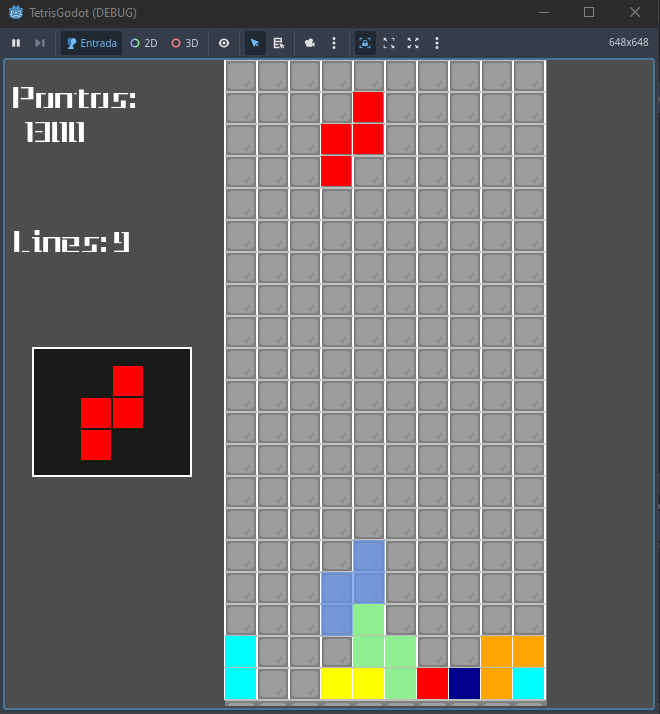
\includegraphics[scale=0.8]{imagens/TetrisGodot.png}
	\\\textbf{Fonte:} Elaborado pelo autor
	\label{fig:godottetris}
\end{figure}
\FloatBarrier

\FloatBarrier
\begin{figure}[!htbp]
	\centering
	\caption{Jogo Tetris na LibGDX}
	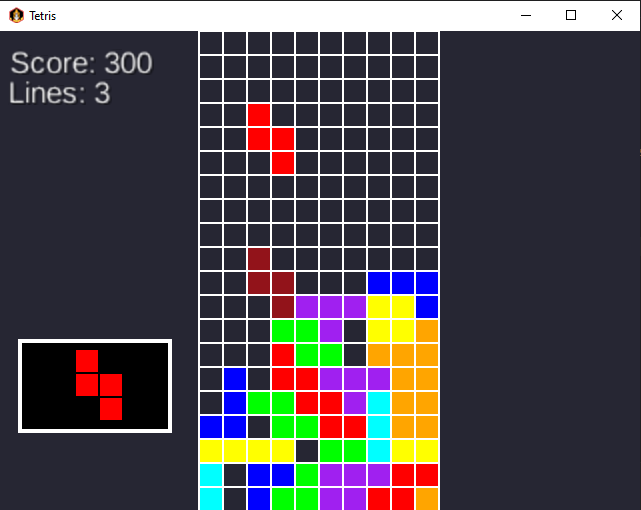
\includegraphics[scale=0.8]{imagens/TetrisLibGDX.png}
	\\\textbf{Fonte:} Elaborado pelo autor
	\label{fig:libgdxtetris}
\end{figure}
\FloatBarrier

\FloatBarrier
\begin{figure}[!htbp]
	\centering
	\caption{Jogo Tetris na Raylib}
	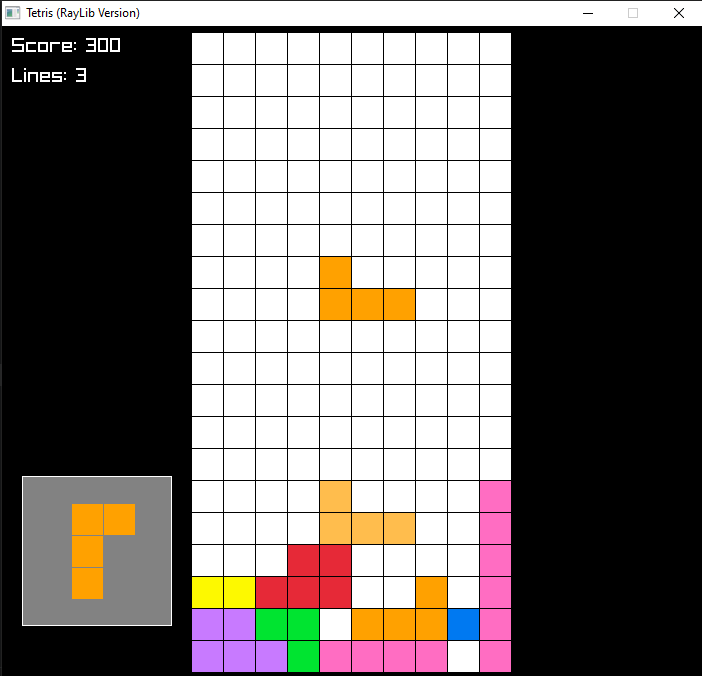
\includegraphics[scale=0.8]{imagens/TetrisRaylib.png}
	\\\textbf{Fonte:} Elaborado pelo autor
	\label{fig:raylibtetris}
\end{figure}
\FloatBarrier

\FloatBarrier
\begin{figure}[!htbp]
	\centering
	\caption{Tetris na Pygame}
	\includegraphics[scale=0.8]{imagens/TetrisPygame.png}
	\\\textbf{Fonte:} Elaborado pelo autor
	\label{fig:pygametetris}
\end{figure}
\FloatBarrier

Todos os códigos-fonte desenvolvidos estão disponibilizados em repositórios públicos na plataforma GitHub. O histórico de commits evidenciam a evolução das implementações.
Abaixo estão os links para os repositórios de cada implementação do jogo \textit{Tetris} utilizando as tecnologias selecionadas:

\begin{itemize}
\item \textbf{Tetris Godot:} \url{https://github.com/Samuskox/Tetris-Godot}
\item \textbf{Tetris LibGDX (Java):} \url{https://github.com/Samuskox/Tetris-LibGDX}
\item \textbf{Tetris Raylib (C++):} \url{https://github.com/Samuskox/Tetris-Raylib}
\item \textbf{Tetris Pygame (Python):} \url{https://github.com/Samuskox/Tetris-Pygame}
\end{itemize}

\subsection{Analise Comparativa}

A análise comparativa entre as tecnologias utilizadas permitiu observar diferenças significativas relacionadas à estrutura de desenvolvimento, modularização do código, facilidade de implementação e nível de abstração oferecido por cada ferramenta. Apesar de todas as tecnologias terem sido capazes de implementar os requisitos funcionais do jogo \textit{Tetris}, cada uma apresentou vantagens e limitações específicas durante o processo de desenvolvimento.

\subsubsection{Facilidade de Desenvolvimento}

A \textit{Godot} e a \textit{Pygame} apresentaram menor complexidade inicial de desenvolvimento, permitindo uma implementação mais rápida das mecânicas básicas do jogo. A estrutura baseada em nós da \textit{Godot} simplificou o gerenciamento dos elementos gráficos e temporizadores, enquanto a flexibilidade da linguagem \textit{Python} tornou o desenvolvimento na \textit{Pygame} mais acessível.

Por outro lado, a \textit{LibGDX} e a \textit{Raylib} exigiram maior configuração inicial e uma organização estrutural mais detalhada, especialmente devido ao uso de linguagens mais robustas como \textit{Java} e \textit{C++}. Entretanto, essas tecnologias proporcionaram maior controle sobre o desenvolvimento do projeto.

\subsubsection{Arquitetura e Modularização}

Durante as implementações, observou-se que a \textit{LibGDX} e a \textit{Raylib} favoreceram uma organização mais modular do código, utilizando separação em múltiplas classes e responsabilidades distintas para entrada do usuário, renderização e lógica do jogo. Em especial, a implementação em \textit{C++} apresentou uma estrutura mais próxima de aplicações de baixo nível, utilizando ponteiros e referências, arquivos de cabeçalho e separação entre declaração e implementação.

A implementação em \textit{Pygame} apresentou uma estrutura mais procedural e linear, reduzindo a complexidade da arquitetura, porém com menor modularização em comparação às demais tecnologias, apesar de ser possível a separação de funções e responsabilidades em diferentes arquivos Python, utilizando importações entre módulos, a flexibilidade da linguagem permite desenvolver sem o uso intensivo de programação orientada a objetos. A \textit{Godot}, por sua vez, apresentou uma abordagem híbrida, utilizando nós e scripts para organizar os componentes do jogo.

\subsubsection{Curva de Aprendizado}

A curva de aprendizado variou significativamente entre as tecnologias analisadas. A \textit{Pygame} apresentou maior facilidade inicial devido à simplicidade da linguagem \textit{Python} e da própria biblioteca. A \textit{Godot} também demonstrou acessibilidade durante o desenvolvimento, principalmente pela documentação e tutoriais de terceiros.

A \textit{LibGDX} exigiu maior compreensão sobre programação orientada a objetos e estruturação de aplicações em \textit{Java}. Já a implementação utilizando \textit{Raylib} e \textit{C++} apresentou a maior complexidade entre as tecnologias estudadas, devido à necessidade de lidar com conceitos mais avançados da linguagem, como ponteiros, referências e organização em arquivos de cabeçalho.



%\david[inline]{sinceramente, não sei se vale pensar em performance. acho que é melhor focar na sua experiência de usar n tecnologias para resolver o mesmo problema. para a quali, pode deixar o que vc coletou abaixo, mas para a defesa, vamos tirar isso. pq se for mesmo analisar desempenho, ai são outros problemas...}

% Com cerca de 70\% do \textit{Tetris} em \textit{Godot} feito é possivel avaliar alguns desempenhos em relação a perfomance da aba monitoramento disponível no \textit{Godot}:

% \begin{itemize}
% 	\item Tempo
% 	\subitem FPS: 34 por segundos
% 	\subitem Processamento: 31.20 ms
% 	\subitem Processo de Física: 0.04 ms
% 	\item Memória
% 	\subitem Estático: 50.82 MiB
% 	\subitem Estático Máximo: 50.89 MiB
% 	\subitem Máx Buf Msg: 4.00 KiB
% 	\item Objetos usados
% 	\subitem Objetos: 1373
% 	\subitem Nós: 6
% 	\item Memória de Vídeo
% 	\subitem Memória de Vídeo: 11.22 MiB
% 	\subitem Memória de Textura: 5.11 MiB
% 	\subitem Memória de Buffer: 6.10 MiB
% \end{itemize}

% Tetris é um jogo simples e leve que não demanda muitos recursos significativos de hardware, 
% portanto os resultados da perfomance não refletem uma carga significativa sobre o desempenho da máquina. Os resultados indicam uma perfomance satisfatória para um estágio que ainda está em desenvolvimento, 
% o FPS médio de 34 é adequado para um projeto em construção, e o tempo de
% processamento (31,20 ms) mostra estabilidade. O consumo de memória e de vídeo está dentro
% de limites esperados, demonstrando boa eficiência no uso dos recursos da engine Godot.

% Até o momento atual, as seguintes atividades foram feitas, abaixo na figura~\ref{fig:cronograma} é mostrado o cronograma das atividades:

% \FloatBarrier
% \begin{figure}[!htbp]
% 	\centering
% 	\caption{Cronograma de Atividades}
% 	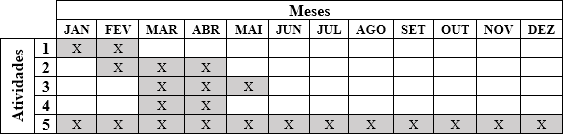
\includegraphics[scale=1]{imagens/cronograma.png}
% 	\\\textbf{Fonte:} feito pelo autor
%     \label{fig:cronograma}
% \end{figure}
% \FloatBarrier

% \begin{enumerate}
% 	\item Estudos de artigos, livros e sites para a fundamentação teórica;
% 	\item Planejamento dos jogos e definição da metodologia;
% 	\item Estudo do motor grafico \textit{Godot} e do ambiente de desenvolvimento;
% 	\item Coleta de Dados;
% 	\item Revisão da documentação.
% \end{enumerate}


% \section{Cronograma do Trabalho}

% Segue abaixo o cronograma de trabalho das atividades realizadas e das que serão executadas até a Avaliação Final de TCC.

% \textbf{Obs:} Para facilitar, crie o cronograma usando o modelo do Word contido no projeto (imagens/templateCronograma.docx), ou qualquer outro \textit{software}, salve a imagem e atualize o arquivo imagens/cronograma.png.

% \FloatBarrier
% \begin{figure*}[!htbp]
% 	\centering
% 	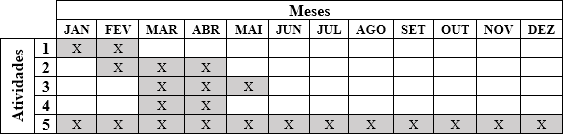
\includegraphics[scale=1]{imagens/cronograma}
% \end{figure*}
% \FloatBarrier

% \begin{enumerate}
% 	\item Descrição da atividade 1;
% 	\item Descrição da atividade 2;
% 	\item Descrição da atividade 3;
% 	\item Descrição da atividade 4;
% 	\item Descrição da atividade 5.
% \end{enumerate}
